\documentclass{beamer}
\usetheme{ConnectivityLab}
\usepackage{times}
\usepackage{graphicx}
\usepackage{verbatim}
\usepackage{outlines}
\usepackage{fancyhdr}
\usepackage{subfigure}
\usepackage{cancel}
\usepackage{bibentry}
\usepackage{varwidth}
\usepackage{etoolbox}
\usepackage{epstopdf}

%%%%%%%%%%%%%%%%%%%%%%%%%%%%%%%%%%%%%%%%%%%%%%%%%%%%%%
%%%%%%%%%%%%%%%%%%%%%%%%%%%%%%%%%%%%%%%%%%%%%%%%%%%%%%

\title {
    EdgeIoT: Mobile Edge Computing for the Internet of Things\cite{7786106}
}
\author {
    Yin-Hong Hsu
}
\date {
    12 11, 2016
}

%%%%%%%%%%%%%%%%%%%%%%%%%%%%%%%%%%%%%%%%%%%%%%%%%%%%%%
%%%%%%%%%%%%%%%%%%%%%%%%%%%%%%%%%%%%%%%%%%%%%%%%%%%%%%

\begin{document}
\begin{frame}
    \titlepage
\end{frame}

%%%%%%%%%%%%%%%%%%%%%%%%%%%%%%%%%%%%%%%%%%%%%%%%%%%%%%
%%%%%%%%%%%%%%%%%%%%%%%%%%%%%%%%%%%%%%%%%%%%%%%%%%%%%%

\begin{frame}{Outline}
    \tableofcontentsgather
    \tableofcontents
\end{frame}

%%%%%%%%%%%%%%%%%%%%%%%%%%%%%%%%%%%%%%%%%%%%%%%%%%%%%%
%%%%%%%%%%%%%%%%%%%%%%%%%%%%%%%%%%%%%%%%%%%%%%%%%%%%%%
\section{Introduction}
\begin{frame} {Introduction} 
    \begin{itemize}
        \item {Today, a tremendous number of IoT device are appeared.}
        \item {Enormous data generated from the distributed IoT devices and transmit to remote cloud.}
        \item \textbf{The smart `'brain`' processing big data via Internet of traditional IoT architecture.} 
    \end{itemize}
\end{frame}

\begin{frame}{Introduction}
    \begin{figure}[t]
        \centering
        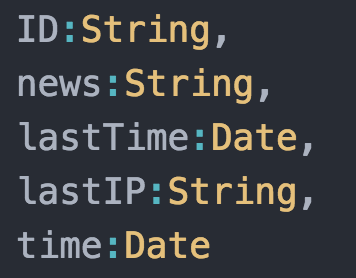
\includegraphics[width=1.1\textwidth]{figures/1.png}
        
    \end{figure}
\end{frame}

\begin{frame} {Introduction} 
    \begin{itemize}
        \item {This paper proposed IoT architecture, edgeIoT with three main ideas as followed.}
        \begin{itemize}
        \item [-]{edgeIoT architecture}
        \item [-]{hierarchical fog computing architecture}
        \item [-]{novel proxy virtual machine migration scheme}
        \end{itemize} 
    \end{itemize}
\end{frame}
%%%%%%%%%%%%%%%%%%%%%%%%%%%%%%%%%%%%%%%%%%%%%%%%%%%%%%
%%%%%%%%%%%%%%%%%%%%%%%%%%%%%%%%%%%%%%%%%%%%%%%%%%%%%%
\section{The EdgeIoT Architecture}
\begin{frame} {The EdgeIoT Architecture} 
    \begin{figure}[t]
        \centering
        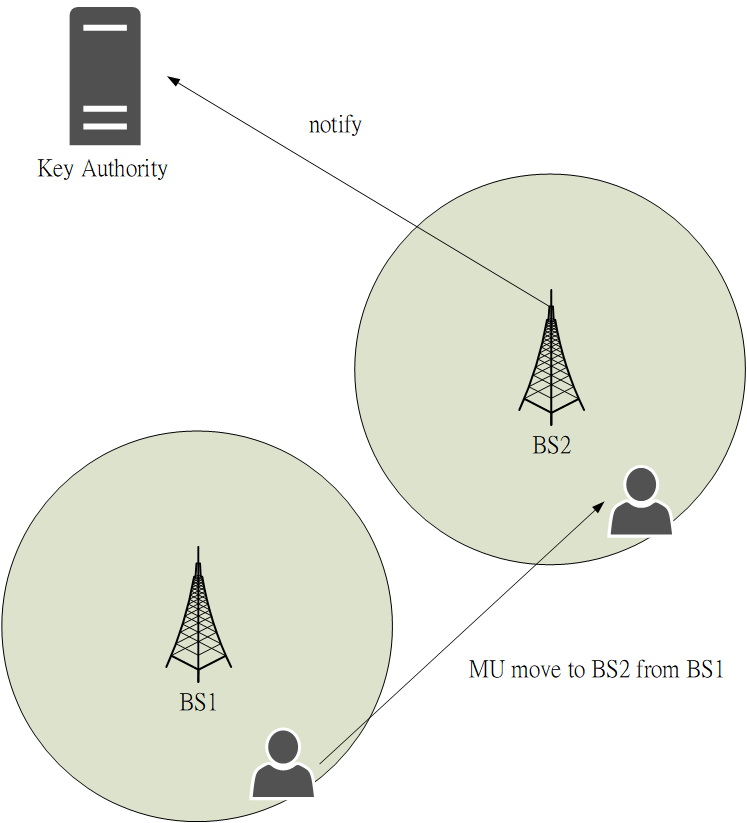
\includegraphics[width=1.1\textwidth]{figures/3.png}
        
    \end{figure}
\end{frame}

\begin{frame} {The EdgeIoT Architecture} 
    \begin{itemize}
         \item {The fog node can be directly connect to BS (local), or deployed at the edge of CN (remote) for different situation.}
    \end{itemize}
\end{frame}

\section{The Hierarchical Fog Computing Architecture}
\begin{frame} {The Hierarchical Fog Computing Architecture} 
    \begin{figure}[t]
        \centering
        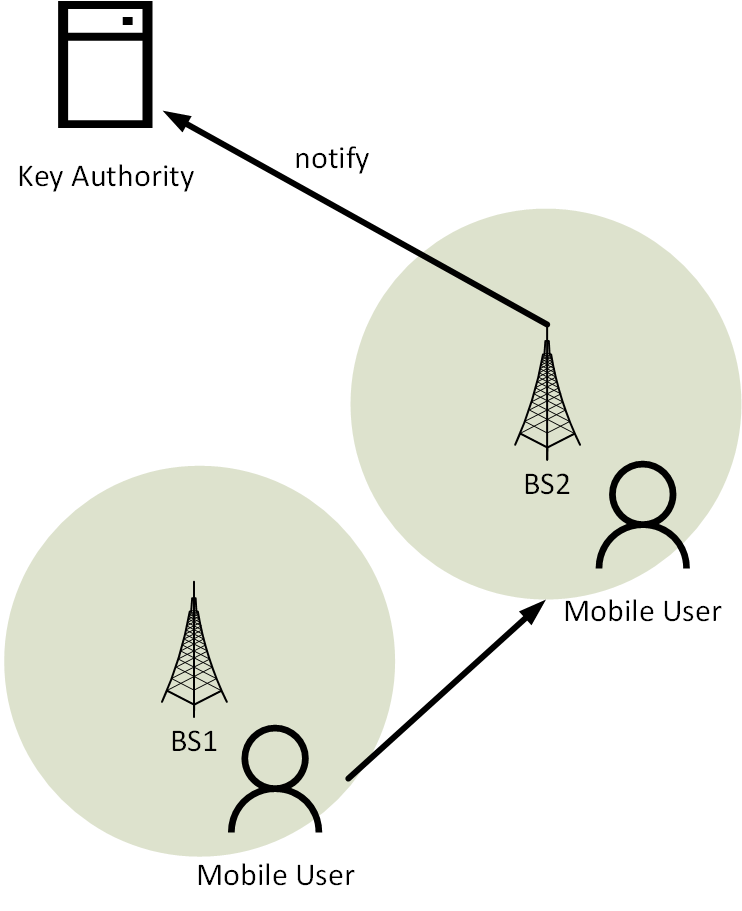
\includegraphics[width=1.1\textwidth]{figures/4.png}
        
    \end{figure}
\end{frame}

\begin{frame} {The Hierarchical Fog Computing Architecture} 
    \begin{itemize}
         \item {Each proxy VM will match to one user.}
         \item {Device belongs to the user have to register to corresponded proxy VM.}
         \item {In proxy VM, the raw data will be processed by semantic model to generate metadata which will pass to application VM and not violate user privacy.}
         \item {For instance, in the terrorist detection application only need timestamp and location rather than the original image.}
    \end{itemize}
\end{frame}

\begin{frame} {The Hierarchical Fog Computing Architecture} 
    \begin{itemize}
         \item {The application VM also can be deployed locally, remotely and as an add-on.}
         \item {Local application VM can be applies to the ParkNet system.}
         \item {Remote application VM can be applies to navigation system.}
         \item {Add-on application VM can be created when some event occur, like terrorist detection system.}
    \end{itemize}
\end{frame}

\begin{frame} {The Hierarchical Fog Computing Architecture} 
    \begin{itemize}
         \item {The location of proxy VM can be allocated dynamically.}
         \item {The proxy VM for mobile device can be decompose from the original one to reduce the E2E delay between device and proxy VM.}
    \end{itemize}
\end{frame}

\begin{frame} {The Hierarchical Fog Computing Architecture} 
    \begin{figure}[t]
        \centering
        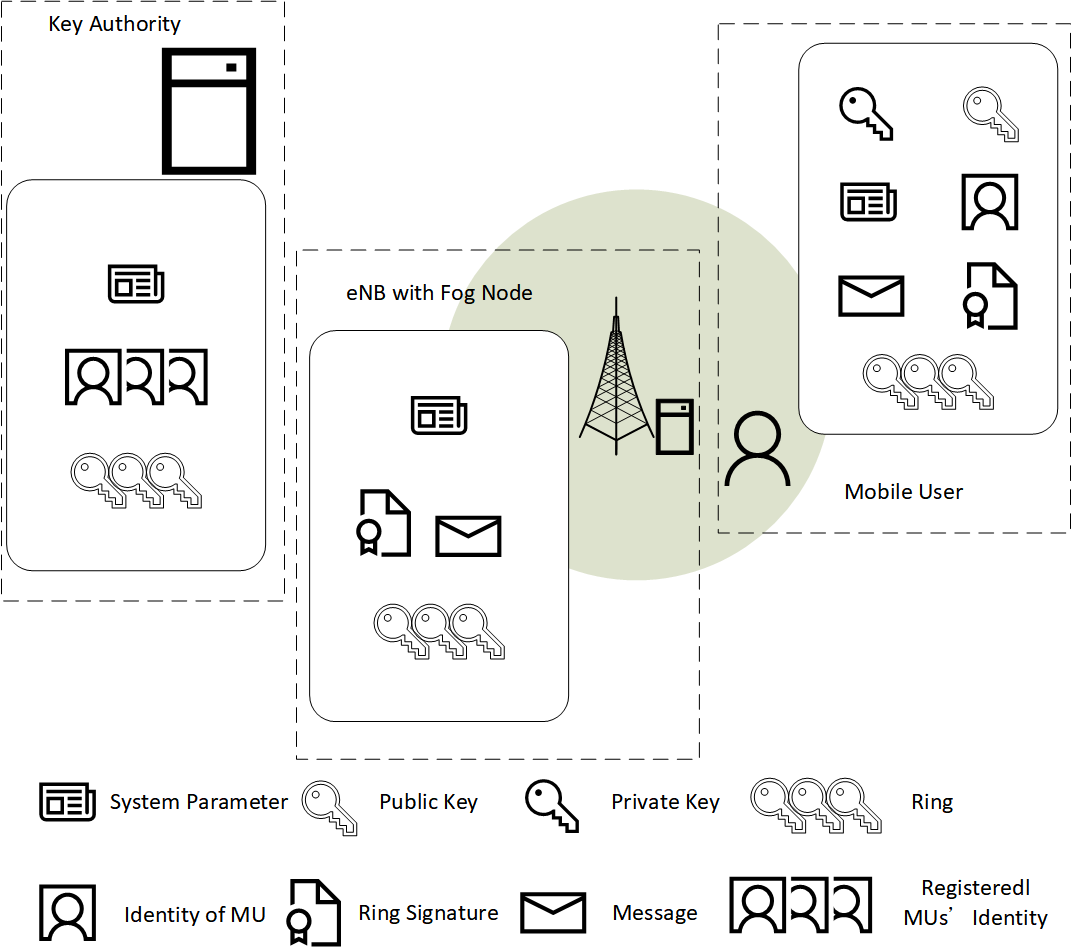
\includegraphics[width=1.1\textwidth]{figures/5.png}
        
    \end{figure}
\end{frame}


\section{Challenges}
\begin{frame} {Proxy VM Mobility Management}
    \begin{itemize}
        \item {When the device roam from BS1 to BS2, it should report it's new location to MME, so that the new proxy VM can be create.}
        \item {There are two mechanisms to update the location for devices:}
        \begin{itemize}
        \item [-]{each device equip a {SIM} card }
        \item [-]{use mobile phone as gateway}
        \end{itemize} 
    \end{itemize}
\end{frame}

\begin{frame} {{IoT} Device Migration Management}
    \begin{itemize}
        \item {As mention before, proxy VM can be decompose and migrated among the fog nodes.}
        \item {It is not necessary to migrate the VM whenever the migration cannot reduce the traffic load.}
    \end{itemize}
\end{frame}

\begin{frame} {{IoT} Device Migration Management} 
    \begin{figure}[t]
        \centering
        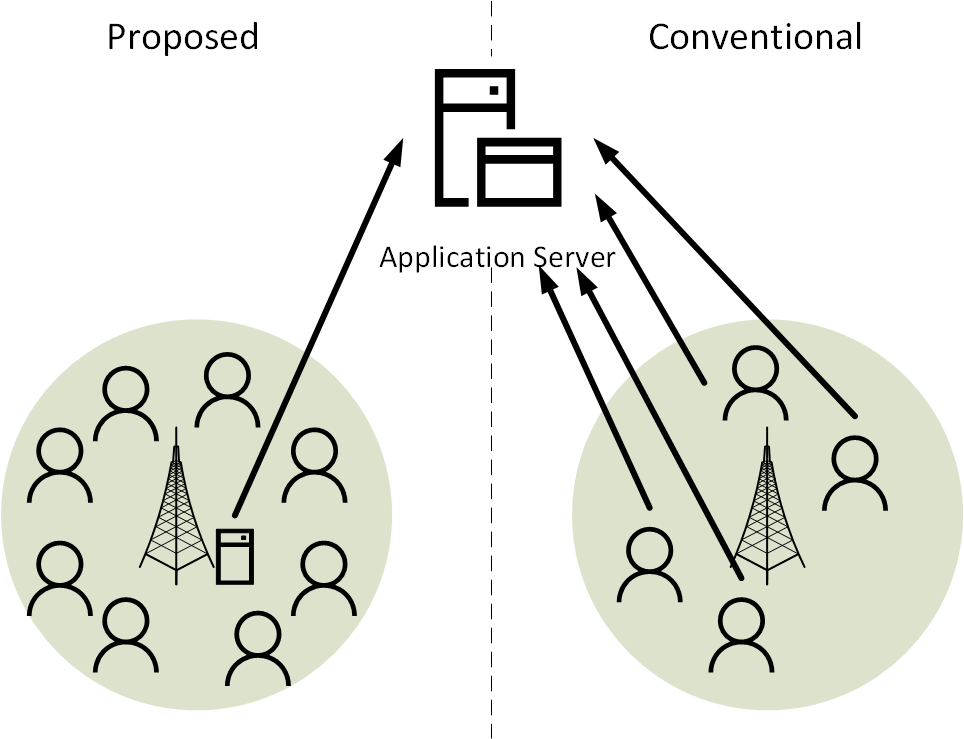
\includegraphics[width=1.0\textwidth]{figures/6.png}
        
    \end{figure}
\end{frame}

\begin{frame} {{IoT} Device Migration Management} 
    \begin{figure}[t]
        \centering
        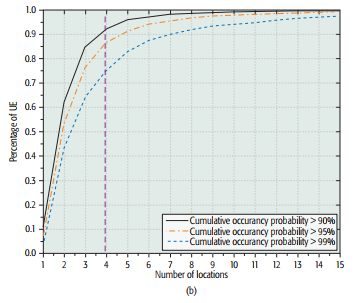
\includegraphics[width=1.0\textwidth]{figures/7.png}
        
    \end{figure}
\end{frame}
%%%%%%%%%%%%%%%%%%%%%%%%%%%%%%%%%%%%%%%%%%%%%%%%%%%%%%
%%%%%%%%%%%%%%%%%%%%%%%%%%%%%%%%%%%%%%%%%%%%%%%%%%%%%%
\section{References}
\calcreferencespagetotal % Calc your References Page total number
\begin{frame}[allowframebreaks]{References}
    \fontsize{9pt}{13}\selectfont
    \bibliographystyle{IEEEtran}
    \bibliography{IEEEabrv,Citation}
\end{frame}

%%%%%%%%%%%%%%%%%%%%%%%%%%%%%%%%%%%%%%%%%%%%%%%%%%%%%%
%%%%%%%%%%%%%%%%%%%%%%%%%%%%%%%%%%%%%%%%%%%%%%%%%%%%%%
\section{}

\begin{frame}
    \centering
    \Large{Thanks for Your Attentions}
\end{frame}

\end{document}
